%%%%%%%%%%%%%%%%%%%%%%%%%%%%%%%%%%%%%%%%%
% Stylish Article
% LaTeX Template
% Version 2.2 (2020-10-22)
%
% This template has been downloaded from:
% http://www.LaTeXTemplates.com
%
% Original author:
% Mathias Legrand (legrand.mathias@gmail.com) 
% With extensive modifications by:
% Vel (vel@latextemplates.com)
%
% License:
% CC BY-NC-SA 3.0 (http://creativecommons.org/licenses/by-nc-sa/3.0/)
%
%%%%%%%%%%%%%%%%%%%%%%%%%%%%%%%%%%%%%%%%%

%----------------------------------------------------------------------------------------
%	PACKAGES AND OTHER DOCUMENT CONFIGURATIONS
%----------------------------------------------------------------------------------------

\documentclass[fleqn,10pt]{SelfArx} % Document font size and equations flushed left

\usepackage[english]{babel} % Specify a different language here - english by default

\usepackage{lipsum,cite} % Required to insert dummy text. To be removed otherwise

\usepackage[T1]{fontenc}
\usepackage[utf8]{inputenc}
\usepackage{newtxtext,newtxmath}

%----------------------------------------------------------------------------------------
%	COLUMNS
%----------------------------------------------------------------------------------------

\setlength{\columnsep}{0.55cm} % Distance between the two columns of text
\setlength{\fboxrule}{0.75pt} % Width of the border around the abstract

%----------------------------------------------------------------------------------------
%	COLORS
%----------------------------------------------------------------------------------------

\definecolor{color1}{RGB}{0,0,90} % Color of the article title and sections
\definecolor{color2}{RGB}{0,20,20} % Color of the boxes behind the abstract and headings

%----------------------------------------------------------------------------------------
%	HYPERLINKS
%----------------------------------------------------------------------------------------

\usepackage{hyperref} % Required for hyperlinks

\hypersetup{
	hidelinks,
	colorlinks,
	breaklinks=true,
	urlcolor=color2,
	citecolor=color1,
	linkcolor=color1,
	bookmarksopen=false,
	pdftitle={Title},
	pdfauthor={Author},
}

%----------------------------------------------------------------------------------------
%	ARTICLE INFORMATION
%----------------------------------------------------------------------------------------

\JournalInfo{Survey Report, 7, Nov, 2024} % Journal information
\Archive{Final Report for AI3605} % Additional notes (e.g. copyright, DOI, review/research article)

\PaperTitle{Opportunities and Challenges of Large Language Models in Industry Applications} % Article title

\Authors{Yuan Gao}
% \Authors{John Smith\textsuperscript{1}} % Authors
% \affiliation{\textsuperscript{1}\textit{}} % Author affiliation



\Keywords{Keyword1 --- Keyword2 --- Keyword3} % Keywords - if you don't want any simply remove all the text between the curly brackets
\newcommand{\keywordname}{Keywords} % Defines the keywords heading name

%----------------------------------------------------------------------------------------
%	ABSTRACT
%----------------------------------------------------------------------------------------

\Abstract{
	In recent years, large language models(LLMs) have gained gained significant attention not only in academic, but also in industry. With the rising demand of the LLMs and the incredible potential interest of the AI-powered applications, it occurs massive opportunities also challenges. These LLMs, including GPT-4, Gemini, Qwen, and other advanced models, have demonstrated there abilities to automate tasks such as writing, coding, analysis and more. They are also transforming fields like healthcare, education, marketing by enabling prominent personalization and efficiency. However, there still exists several challenges performing as obstacles to the development of LLMs, including data privacy, ethics, cost and more. In this survey, we will explore and discuss about both opportunities and chanllenges of LLMs in industrial applications, providing insights into current research and future directions for addressing these obstacles.
}

%----------------------------------------------------------------------------------------



\begin{document}

\maketitle % Output the title and abstract box

\tableofcontents % Output the contents section

\thispagestyle{empty} % Removes page numbering from the first page

%----------------------------------------------------------------------------------------
%	ARTICLE CONTENTS
%----------------------------------------------------------------------------------------

\section*{Introduction} % The \section*{} command stops section numbering

\addcontentsline{toc}{section}{Introduction} % Adds this section to the table of contents

% paragraph 1 : Briefly introduce the concept and background of large language models (LLMs)

% paragraph 2 : Explain the importance and influence of LLMs in the field of artificial intelligence

% paragraph 3 : Outline the objectives and structure of the report

% \lipsum[1-3] % Dummy text
%  and some mathematics $\cos\pi=-1$ and $\alpha$ in the text\footnote{And some mathematics $\cos\pi=-1$ and $\alpha$ in the text.}.

The field of natural language processing (NLP) has changed a lot with the rise of large language models (LLMs). Coming from years of research in computational linguistics and deep learning, LLMs are based on early work like the use of neural networks for language modeling in the late 1990s and the transformer-based architectures introduced by Vaswani et al. \cite{Vaswani:2017at}. These steps led to the creation of models like GPT \cite{Radford:2018tf}, BERT \cite{Devlin:2018br}, and, more recently, GPT-4, Gemini, and Qwen, which now surpass humans in many language tasks.

In the beginning, LLMs were praised in academic settings for advancing research in linguistics and machine learning. Their uses were mostly experimental, focusing on benchmarks and competitions like GLUE and SuperGLUE. But as models grew larger and AI-powered tools became more common, their use spread beyond academia. Now, industries like healthcare and marketing use LLMs to transform their work. These models help automate tasks like creating content, programming, and making decisions.

\begin{figure}[ht]\centering
	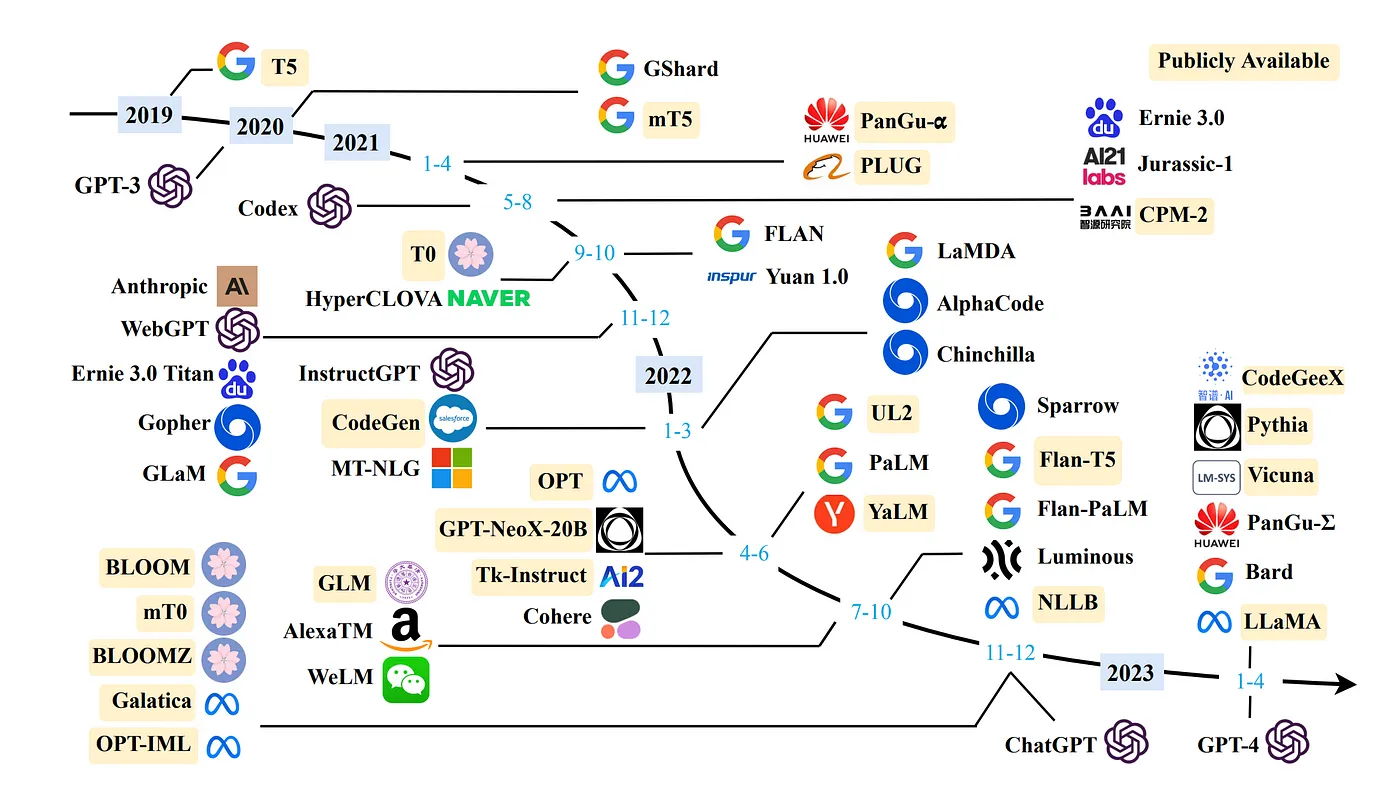
\includegraphics[width=\linewidth]{Figures/development.png}
	\caption{Chronological development of large language models (LLMs) from 2019 to 2023.}
	\label{fig:dev}
\end{figure}

After the coming of GPT-3, the whole industry make sense that the era of LLMs are coming. From 2020 to now, industry release their LLMs like mushrooms after rain, few of them make a significant success including Claude, Gemini, Ernie, LLaMA. While others are still trying their best to make their LLMs outstanding. We can briefly grasp the development context by Figure\ref{fig:dev}

Even with their promise, using LLMs in industries comes with challenges. Problems like data privacy, ethical concerns, and the high cost of running these models often slow their wider use \cite{Bender:2021ai}. These issues not only limit their usefulness but also show gaps in research and implementation.

This survey aims to connect advances in research with real-world applications of LLMs. By collecting input from professionals and researchers, the study looks to find ways to use LLMs better in industries while addressing the problems that hold them back. The results aim to add to the discussion about AI’s role in society and offer useful ideas for researchers, policymakers, and business leaders.

%------------------------------------------------

\section{Overview of Core-tech in LLMs}

% \begin{figure*}[ht]\centering % Using \begin{figure*} makes the figure take up the entire width of the page
% 	
\includegraphics[width=\linewidth]{view}
% 	\caption{Wide Picture}
% 	\label{fig:view}
% \end{figure*}

% \lipsum[4] % Dummy text

% \begin{equation}
% 	\cos^3 \theta =\frac{1}{4}\cos\theta+\frac{3}{4}\cos 3\theta
% 	\label{eq:refname2}
% \end{equation}

% \lipsum[5] % Dummy text

% \begin{enumerate}[noitemsep] % [noitemsep] removes whitespace between the items for a compact look
% 	\item First item in a list
% 	\item Second item in a list
% 	\item Third item in a list
% \end{enumerate}



% \lipsum[6] % Dummy text

\subsection{Objective of Language Modeling}

Large Language Models (LLMs) predict the probability of natural language sequences. Specifically, they compute the probability of the next word \(w_t\) based on previous words. This is expressed as:
\[
P(w_t | w_1, w_2, \ldots, w_{t-1}).
\]
For a full sequence \(W = (w_1, w_2, \ldots, w_T)\), the model maximizes the likelihood function during training:
\[
\mathcal{L}(\theta) = \sum_{t=1}^T \log P(w_t | w_1, w_2, \ldots, w_{t-1}; \theta).
\]
Here, \(\theta\) represents the model parameters.

\subsubsection{Transformer Architecture}

Transformer architecture is a neural network model. It has significantly impacted natural language processing (NLP). Unlike traditional recurrent neural networks (RNNs), transformers use an attention mechanism. This mechanism helps the model focus on important parts of the input sequence. This helps the model capture long-range dependencies. As a result, transformers perform better in various NLP tasks. 

\begin{figure}[ht]\centering
	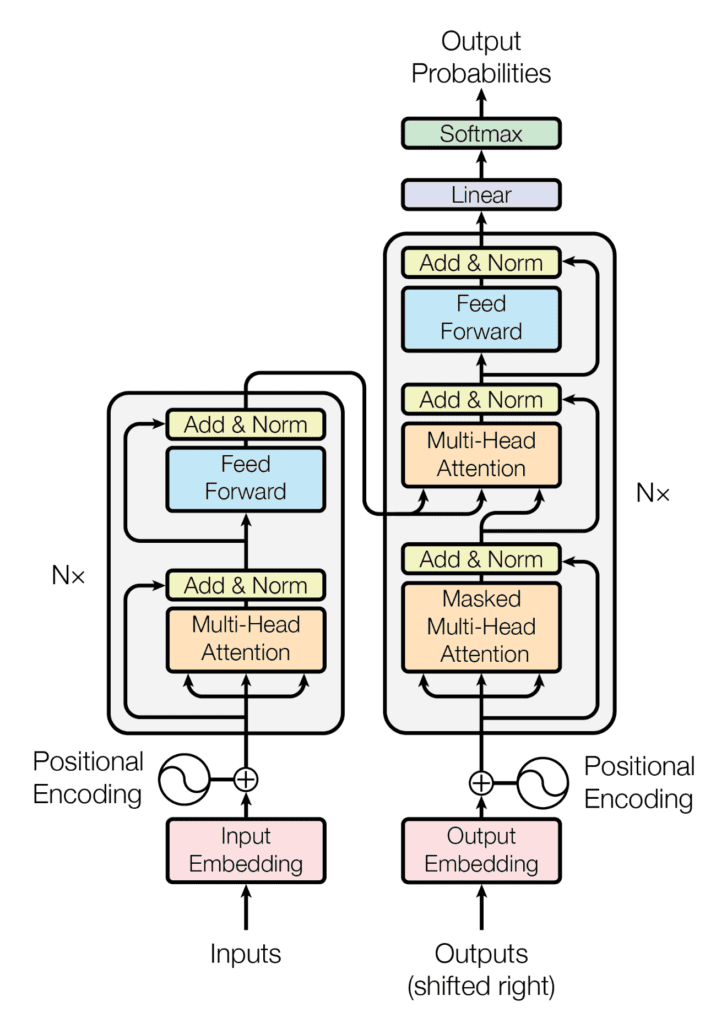
\includegraphics[width=0.3\textwidth]{Figures/attention.png}
	\caption{The  encoder-decoder structure of the Transformer architecture
	Taken from “Attention Is All You Need“\cite{vaswani2023attentionneed}}
	\label{fig:tran}
\end{figure}

\subsubsection{Self-Attention Mechanism}

The self-attention mechanism identifies the importance of input tokens relative to each other. For an input sequence \(X \in \mathbb{R}^{n \times d}\), where \(n\) is the sequence length and \(d\) is the embedding dimension, the process follows these steps:
\begin{enumerate}
    \item Compute query \(Q\), key \(K\), and value \(V\) matrices:
    \[
    Q = XW_Q, \quad K = XW_K, \quad V = XW_V,
    \]
    where \(W_Q, W_K, W_V \in \mathbb{R}^{d \times d_k}\) are trainable weight matrices.
    \item Calculate attention scores:
    \[
    \text{Attention}(Q, K, V) = \text{softmax}\left(\frac{QK^\top}{\sqrt{d_k}}\right)V.
    \]
    The \(\sqrt{d_k}\) term normalizes the dot product to improve stability.
\end{enumerate}

\subsubsection{Multi-Head Attention}

Multi-head attention enhances the model's ability to learn diverse patterns. It divides self-attention into multiple parallel "heads." The output is:
\[
\text{MultiHead}(Q, K, V) = \text{Concat}(\text{head}_1, \text{head}_2, \ldots, \text{head}_h)W_O,
\]
where each head is:
\[
\text{head}_i = \text{Attention}(QW_{Q_i}, KW_{K_i}, VW_{V_i}).
\]
Here, \(W_{Q_i}, W_{K_i}, W_{V_i} \in \mathbb{R}^{d \times d_k}\) are weight matrices, and \(W_O \in \mathbb{R}^{hd_k \times d}\) combines the outputs.

\subsubsection{Positional Encoding}

Transformers do not have recurrence. To handle token order, positional encoding is added to the input embeddings. With sinusoidal encoding, for position \(t\) and dimension \(i\):
\[
PE(t, 2i) = \sin\left(\frac{t}{10000^{2i/d}}\right), \quad PE(t, 2i+1) = \cos\left(\frac{t}{10000^{2i/d}}\right).
\]

\subsection{Feed-Forward Neural Network (FFN)}

Each transformer layer includes a feed-forward neural network. It applies a non-linear transformation to each token independently:
\[
\text{FFN}(x) = \text{ReLU}(xW_1 + b_1)W_2 + b_2,
\]
where \(W_1, W_2\) are weight matrices, and \(b_1, b_2\) are biases.

\subsection{Training Objective}

LLMs are trained using the negative log-likelihood of the true sequence:
\[
\mathcal{L}(\theta) = -\sum_{t=1}^T \log P_\theta(w_t | w_1, w_2, \ldots, w_{t-1}).
\]
The model computes \(P_\theta(w_t | \cdot)\) using the softmax function:
\[
P_\theta(w_t | \cdot) = \frac{\exp(z_t)}{\sum_{w' \in \mathcal{V}} \exp(z_{w'})}.
\]
Here, \(z_t\) are the logits for token \(w_t\), and \(\mathcal{V}\) is the vocabulary.

\subsection{Optimization}

The model parameters are optimized using stochastic gradient descent (SGD) or its variants, like Adam. The gradient of the loss with respect to parameters \(\theta\) is:
\[
\frac{\partial \mathcal{L}}{\partial \theta} = \sum_{t=1}^T \frac{\partial \log P_\theta(w_t | w_1, w_2, \ldots, w_{t-1})}{\partial \theta}.
\]
The parameters are updated iteratively:
\[
\theta \leftarrow \theta - \eta \frac{\partial \mathcal{L}}{\partial \theta},
\]
where \(\eta\) is the learning rate.

\subsection{Scaling and Fine-Tuning}
Fine-tuning is a technique that we use to adapt a pre-trained LLM to a specific task or domain. This allow us to train pre-trained LLM on a smaller, field-specific dataset, which can make the LLMs behave well in the specific domain. By fine-tuning, we can improve the model's performance, and more inspiringly, we can make experts in any specific field.

LLM performance improves with scaling. Key scaling strategies include:
\begin{itemize}
    \item \textbf{Depth}: Increase the number of transformer layers.
    \item \textbf{Width}: Use larger embedding dimensions.
    \item \textbf{Data}: Train on large-scale text corpora.
\end{itemize}

By the escalation of the factors we mentioned above, LLM can grow stronger and stronger. Figuratively, LLM is just like a child who is learning to speak. With more knowledge(data), bigger brain(width), the child will become more and more smart. This is so called \textbf{Scaling Laws}, which is one of the most important factors that cause the rapid development and potential issues of LLM.




% \subsection{Architectures}

% \lipsum[9] % Dummy text

% \begin{figure}[ht]\centering
% 	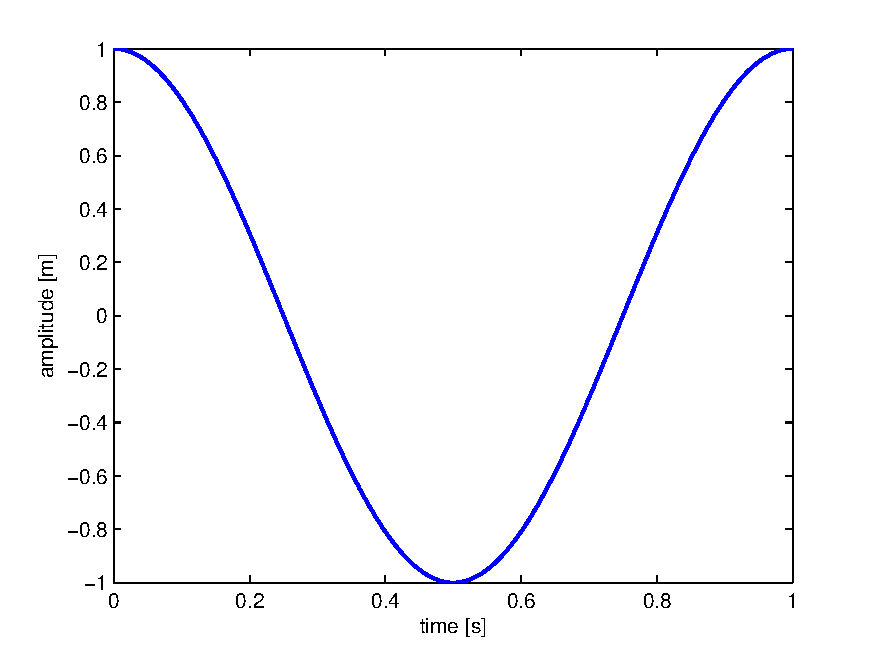
\includegraphics[width=\linewidth]{results}
% 	\caption{In-text Picture}
% 	\label{fig:results}
% \end{figure}

% Reference to Figure \ref{fig:results}.

% it depends
% \subsection{Potential Issues}
%------------------------------------------------

\section{Industry Application Scenarios}

With the development of LLM, there has been a various fields that embed LLM into their own applications. Here we will introduce some of the most common application scenarios.
% \lipsum[10] % Dummy text

\subsection{Content Creation}

\paragraph{Script Writing} Film script writing is a creative process that combines art and skills, which traditionally requires a deep background and practical accumulation. Today, artificial intelligence and big data technologies have effectively improved its efficiency and quality. Recently, The Shanghai Jiao Tong University team proposed using the Large Language Model (LLM) to realize interactive drama \cite{wu2024roleplay}, a new art form that combines traditional drama with modern AI technology. By redefining the six elements of drama, the audience can interact with the characters, explore and influence the development of the plot, and gain a richer experience.




\subsection{Chatbot}

\paragraph{Customer Support} Using LLMs' powerful language capabilities, it's efficient to integrate specific knowledge, speaking manner, and other required information into chatbots. Therefore, chatbots can perfectly play the role of customer service staff. For example, Wofeng Technology provides Bayer (China)'s virtual medical representative platform with intelligent customer service products supported by AI big models, completing the AI empowerment of intelligent virtual representatives in the enterprise WeChat channel, thereby creating an intelligent customer service system for the expert community of the Academy of Imaging, helping Bayer (China) achieve a doubles model growth rate far higher than the offline representative singles and the industry average, academic refined operations with high recognition from doctors, access to nearly 100 hospitals throughout the year, and the formation of a discipline circle to continuously promote other products.

\begin{figure}[ht]\centering
	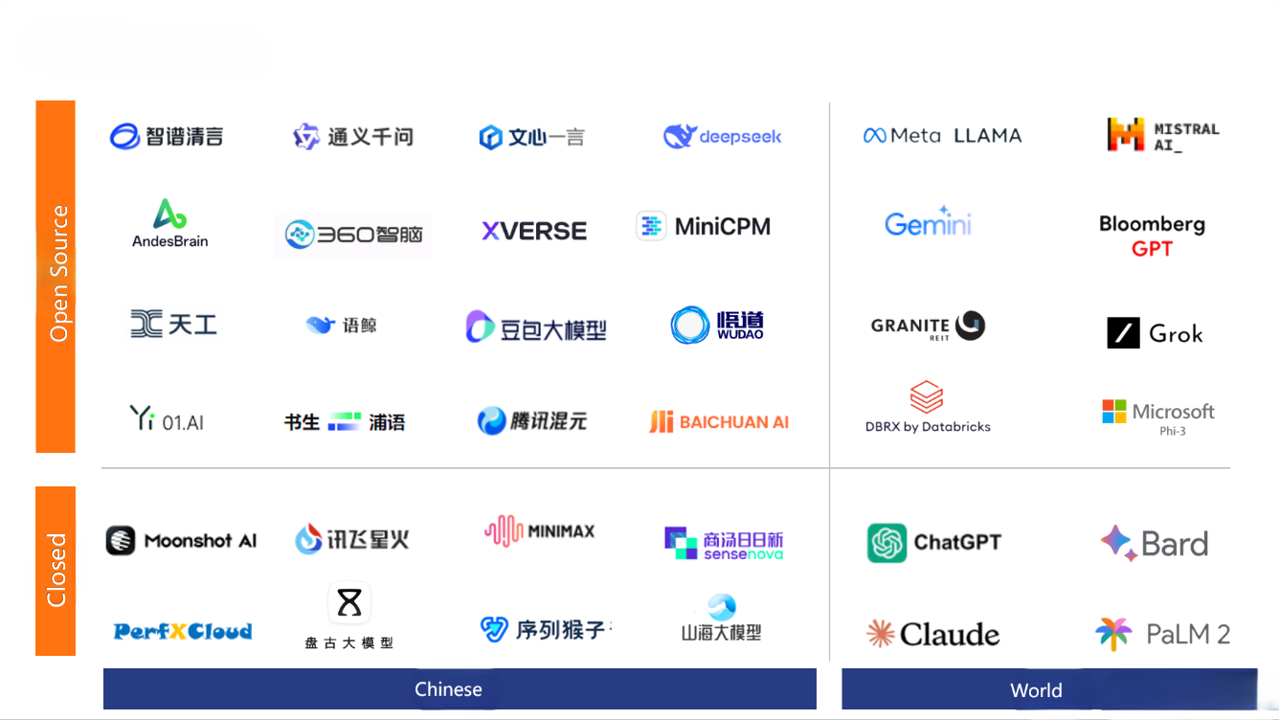
\includegraphics[width=\linewidth]{Figures/LLMs.png}
	\caption{Various LLM applications around world}
	\label{fig:llmapp}
\end{figure}

\paragraph{Q\&A Systems} When someone first encounter the LLM, if you ask them how to use it, the intuition will tell that Q\&A systems are born for LLM. Figure \ref{fig:llmapp} shows almost all of the current Q\&A systems that are based on LLMs. The flourish of Q\&A systems tells everything.

\subsection{Healcare}

\paragraph{Diagnostic Assistance} On September 19, 2023, Baidu released the Chinese first “industrial-grade” large medical model - the "Lingyi(Great Doctor)" big model based on LLM. In terms of diagnosis assistance, Baidu Lingyi Big Model provides doctors with efficient and accurate tools through functions such as medical record generation, patient condition briefing, intelligent question and answer, and clinical decision support. For example, it can automatically generate standardized medical records, extract key diagnosis and treatment information, answer professional questions based on authoritative literature, and connect with hospital systems to optimize workflows, thereby greatly improving medical service efficiency and diagnosis quality.

\paragraph{Pharmaceutical} Huawei Cloud Pangu Drug Molecular Model has performed well in tasks such as molecule generation, property prediction and optimization by learning massive amounts of drug molecular data, greatly improving the efficiency of new drug research and development, shortening the research and development cycle and reducing costs. For example, the model helped develop broad-spectrum antibacterial drugs, shortening the research and development cycle from several years to one month and reducing costs by 70\%, providing strong support for the intelligent transformation of the pharmaceutical industry.




\subsection{Education}

\paragraph{Personalized Learning} In 2023, Chinese education technology companies actively applied big models in the field of education and launched a number of innovative applications to improve teaching and learning effects through intelligent means. In July, NetEase Youdao released the big model "Zi Yue" for K12 education, which accomplishes personalized analysis guidance, guided learning and other functions. The big model can better teach students in accordance with their aptitude and provide students with all-round knowledge support. In August, TAL Education Technology released their big model MathGPT in the field of mathematics, which can automatically generate questions and give answers, covering elementary school to high school mathematics knowledge. 

LLMs in the field of education are becoming a new tool for intelligent assisted teaching. Their knowledge integration capabilities can meet the dynamic needs of students, realize personalized learning, and improve the quality of teaching together with teachers.

\paragraph{Language Learning} Named Large Language Models, LLMs are born to be brilliant in language field, which can be proved by the fact that the first batch of embedding LLMs into industrial applications is professional language teaching institutions like Duolingo. As early as 2021, before ChatGPT formally published, Duolingo has embeded GPT-3 into their language-teaching application to help generate learning content. As LLMs growing more and more powerful, now it can be used in many scenarios including DIY learning content, making personalized learning plans, helping students to improve their writing skills, and thanks to MLLMs(multi-modal LLMs), it can even be used to talk with learners and help them to improve their listening and oral skills.

\subsection{Finace}


\paragraph{Financial Analysis} With wide range of financial data accumulated over past 40 years, Bloomberg released BloombergGPT, a LLM specifically designed for financial analysis. Because of the combination of powerful base model and high-quality finacial data, BloombergGPT behaves incredible in financial analysis tasks just like an experienced experts. This applications help to reduce the workload of financial analysts and improve the efficiency.





% \lipsum[11] % Dummy text

% \begin{table}[hbt]
% 	\caption{Table of Grades}
% 	\centering
% 	\begin{tabular}{llr}
% 		\toprule
% 		\multicolumn{2}{c}{Name} \\
% 		\cmidrule(r){1-2}
% 		First name & Last Name & Grade \\
% 		\midrule
% 		John & Doe & $7.5$ \\
% 		Richard & Miles & $2$ \\
% 		\bottomrule
% 	\end{tabular}
% 	\label{tab:label}
% \end{table}



% \lipsum[12] % Dummy text

% \begin{description}
% 	\item[Word] Definition
% 	\item[Concept] Explanation
% 	\item[Idea] Text
% \end{description}

% \subsubsection{Subsubsection}

% \lipsum[13] % Dummy text

% \begin{itemize}[noitemsep] % [noitemsep] removes whitespace between the items for a compact look
% 	\item First item in a list
% 	\item Second item in a list
% 	\item Third item in a list
% \end{itemize}

% \subsubsection{Subsubsection}

% \lipsum[14] % Dummy text

\section{Opportunities}

\subsection{Ehancing Efficiency}
\subsection{Improving Quality}
\subsection{Expanding Market Scale}
\subsection{Personalized Service}

\section{Challenges}
example: IBM Watson's failure
\subsection{Data Privacy}
\subsection{Data Resources}
\subsection{Ethics \& Bias}
\subsection{Costs}
\subsection{Regulatory \& Legal Risks}
\subsection{Technical Limitations}
In this part, we can introduce RAG as an optional method to enhance LLM but still some issues
\section{Conclusion}

%expectations, conclusions, suggestions, etc.
\lipsum[15-23] % Dummy text

%------------------------------------------------

\phantomsection
\section*{Acknowledgments} % The \section*{} command stops section numbering

\addcontentsline{toc}{section}{Acknowledgments} % Adds this section to the table of contents

So long and thanks for all the fish \cite{Figueredo:2009dg, Smith:2012qr}.

%----------------------------------------------------------------------------------------
%	REFERENCE LIST
%----------------------------------------------------------------------------------------

\phantomsection
\bibliographystyle{unsrt}
\bibliography{sample.bib}

%----------------------------------------------------------------------------------------

\end{document}